En inverterende opamp snur negativt signal til positivt og motsatt.

\begin{figure}[H]
  \caption{inverterende forsterker}
  \centering
  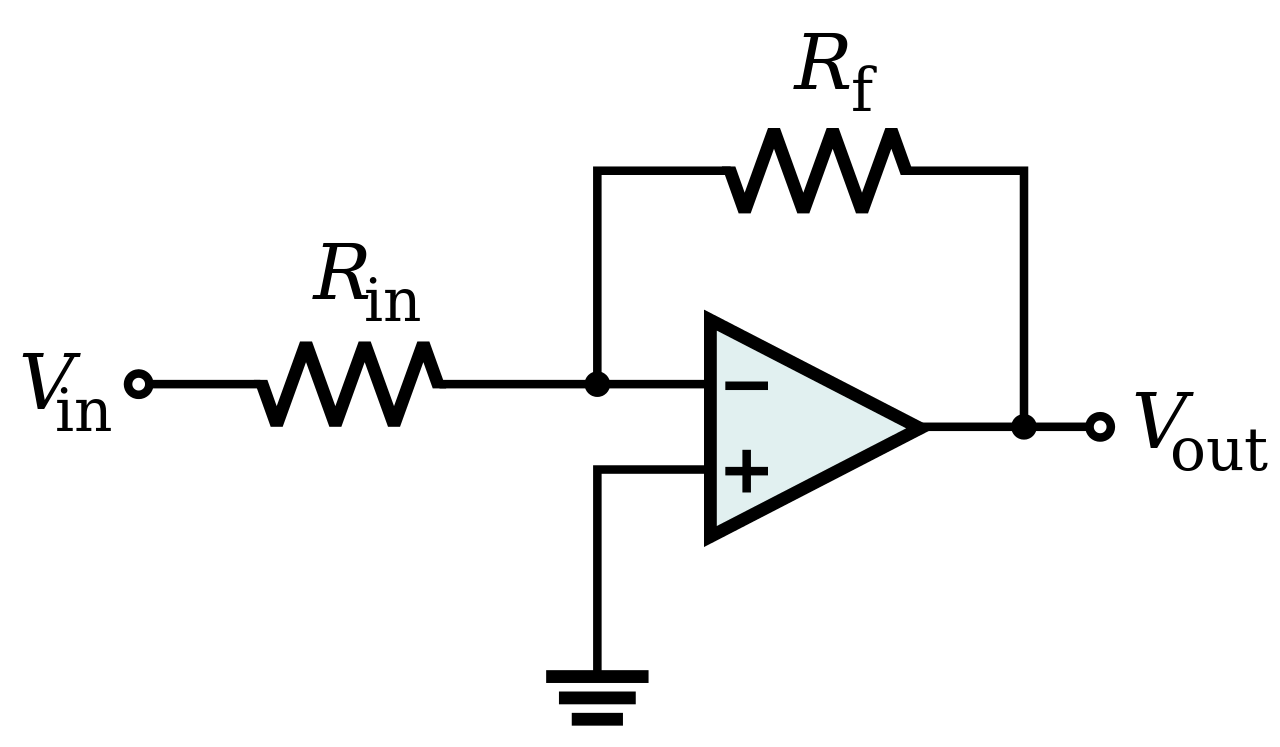
\includegraphics[width=\textwidth]{./img/opamp-invert}
\end{figure}

Forsterkningen er gitt ved
$$A_{vf} = \frac{V_{out}}{V_{in}}$$
Dette kan forenkles når $A_v >> 1$ til
$$A_{vf} = -\frac{R_f}{R_{in}}$$

Vi kan også finne $v_i$
$$v_i = \frac{v_o}{A_v}$$

Inngangen på en inverterende opamp kan regnes som et \emph{virtuelt nullpunkt}.
